\documentclass{report}
\usepackage{setspace}
%\usepackage{subfigure}

\pagestyle{plain}
\usepackage{amssymb,graphicx,color}
\usepackage{amsfonts}
\usepackage{latexsym}
\usepackage{a4wide}
\usepackage{amsmath}

\usepackage[super]{nth}  % To format ordinal numbers e.g. 1st, 2nd, 3rd, 4th, etc.
\usepackage{enumitem}  % Remove spaces before an enumerate
\usepackage[style=ieee, sorting=none]{biblatex}  % BibTeX  
\usepackage{url}  % urls
\usepackage{listings}  % code snippets
\usepackage{longtable}  % tables
\usepackage{tabu}  % tables
\usepackage{textcomp}  % symbols

\newtheorem{theorem}{THEOREM}
\newtheorem{lemma}[theorem]{LEMMA}
\newtheorem{corollary}[theorem]{COROLLARY}
\newtheorem{proposition}[theorem]{PROPOSITION}
\newtheorem{remark}[theorem]{REMARK}
\newtheorem{definition}[theorem]{DEFINITION}
\newtheorem{fact}[theorem]{FACT}

\newtheorem{problem}[theorem]{PROBLEM}
\newtheorem{exercise}[theorem]{EXERCISE}
\def \set#1{\{#1\} }

\newenvironment{proof}{
PROOF:
\begin{quotation}}{
$\Box$ \end{quotation}}



\newcommand{\nats}{\mbox{\( \mathbb N \)}}
\newcommand{\rat}{\mbox{\(\mathbb Q\)}}
\newcommand{\rats}{\mbox{\(\mathbb Q\)}}
\newcommand{\reals}{\mbox{\(\mathbb R\)}}
\newcommand{\ints}{\mbox{\(\mathbb Z\)}}

\setcounter{secnumdepth}{3}  % Add numbering to \subsubsection
\setcounter{tocdepth}{3}  % Include \subsubsection in ToC
\setlist{nosep}  % Remove spaces before an enumerate
\setlength{\LTpre}{1em}  % remove spaces before longtable
\setlength{\LTpost}{0em}  % remove spaces after longtable
\newcommand{\textapprox}{\raisebox{0.5ex}{\texttildelow}}  % '~' sign

\bibliography{bibliography.bib}  % Load bibliography

%%%%%%%%%%%%%%%%%%%%%%%%%%


\title{{\vspace{-14em} 
\includegraphics[scale=0.4]{ucl_logo.png}}\\
{{\Huge Using natural language processing to develop a pipeline to analyse media representation of people with disabilities in Web-based news articles}}\\
{\large Collection and filtering of Web-based news articles, comparison of open-source sentiment models, and applications of the technology
}\\
}
\date{Submission date: \nth{30} April 2018}
\author{Bagus Maulana\thanks{
{\bf Disclaimer:}
This report is submitted as part requirement for the MEng Degree in Computer Science at UCL. It is
substantially the result of my own work except where explicitly indicated in the text.
\emph{The report may be freely copied and distributed provided the source is explicitly acknowledged}}
\\ \\
MEng Computer Science\\ \\
Catherine Holloway, Nicholas Firth}



\begin{document}
 
\onehalfspacing
\maketitle
\begin{abstract}

\textbf{Report Title:}  Using natural language processing to develop a pipeline to analyse media representation of people with disabilities in Web-based news articles: Collection and filtering of Web-based news articles, comparison of open-source sentiment models, and applications of the technology

\textbf{Author’s Name:} Bagus Maulana

\textbf{Supervisor’s Name:} Catherine Holloway, Nicholas Firth

\textbf{Date and Year of Submission:} \nth{30} April 2018\\

Analyses of news media, and representation of groups such as people with disabilities, is a popular research theme in various fields. A common approach is to manually analyse a sample of a few hundred news articles and generalise, but computational natural language processing (NLP) can be used to process articles much faster and vastly increase the sample size, to uncover in-depth information such as trends over time and between different publishers. This project explores the feasibility of developing a computational pipeline that performs data collection (from online news sources), filtering, parsing, sentiment scoring, and statistical analysis to reveal these trends. Results indicate that for some metrics (such as moving average of sentiment score) and on certain keyword categories, minor trends over time and between different publishers are apparent, although inconsistent; but there are still room for improvement, such as by training a domain-specific sentiment scorer with labelled data to improve score accuracy (consistency).
% Python, NumPy, SciPy, scikit-learn, matplotlib, NLTK, SpaCy, VADER
% todo placeholder - delete this later and replace with the three paragraphs defined below

%% Three paragraphs:

%% What the project is about, the principle aims and goals, and specific challenges.

%% How you carried out the project and what work it involved. How you went about meeting the project goals.

%% The results and achievements of the project. What the outcome is.

%% Half a page’s length.}
\end{abstract}
\tableofcontents
\setcounter{page}{1}


\chapter{Introduction} \label{Introduction} % 2-4 pages

%% Outline the problem you are working on, why it is interesting and what the challenges are.

% Talk about NLP
Natural language processing (NLP) encompasses a wide range of computational techniques for machine understanding of human (natural) language that are often used alongside each other.
The review article \cite{cambria2014jumping} defines natural language processing as 'a theory-motivated range of computational techniques for the automatic analysis and representation of human language.'
The techniques that fall under the umbrella natural language processing include word tokenisation, probabilistic language modelling, translation, part-of-speech parsing, sentiment analysis (or opinion mining), text classification/categorisation, and topic modelling, among other things.
The computational models used in natural language processing range from simple rule-based models (e.g. splitting a sentence on whitespace to tokenise words) to statistical machine learning and deep learning models.
Natural language processing is now applied for various everyday technologies, for example, information retrieval for search engines such as Google and Bing, and categorisation and topic modelling for recommendation engines used to suggest 'similar' articles.

The obvious advantage of natural language processing is that machines can process vast bodies of human-created literature (books, articles, posts, e-mails, messages, etc.) much faster than humans can, processing thousands or millions of documents per second. 
This allows for high-level quantitative analyses of all documents in a vast corpora for a given domain to be feasible, which can uncover information previously inaccessible by only reading and generalising from a small sample of documents.
For example, this level of quantitative analysis can uncover trends and patterns within a given domain (e.g. how does the popularity of the term 'mentally ill' increase or decrease year-on-year in English news media?). 

% Other work in using NLP for media analysis
Various other studies have attempted to utilise natural language processing to perform high-level analyses in the domain of news media.
The research done in \cite{lansdall2017content} assembled a vast corpus of regional newspapers in the United Kingdom spanning 150 years to detect long-term patterns of cultural change (e.g. increase of female representation in the news, or when trains overtook horses for transportation) by analysing n-gram trends and named entities. 
More specifically, in the domain of media representation of specified groups of people, studies such as \cite{waseem2016you} has attempted to use features based on natural language processing (such as n-grams and part-of-speech tags) to classify racist and sexist posts in social media, although there is still a research gap in this area (especially for news articles, and/or relating to specific groups, such as people with (specific) disabilities or mental illnesses).
% Just give a short summary, expand this later in Chapter 2

% Why is it interesting & what the challenges are
Applying natural language processing to perform meta-analyses over large text corpora has various interesting potential applications in improving our understanding of the human world - for example, to detect macroscopic cultural shifts as in \cite{lansdall2017content}.
In particular, the representation of specific groups, such as people with disabilities, has been a popular research theme for psychologists, sociologists, and others.
For example, the paper \cite{coverdale2002depictions} analysed a sample of 600 print articles relating to mental illnesses in New Zealand and categorised them to positive and negative depictions, and the predominant themes thereof (e.g. criminality (negative), educational accomplishments (positive)).
Applying natural language processing to this area of research would allow the possibility of discovering higher-level trends, by computationally analysing a much larger sample of articles and identify trends by varying independent variables such as year of publication and publisher.
In this research, a sample of 305,185 news articles (48,967 after filtering off-topic articles) from British online news sources are used.
However, challenges remain as syntax-based statistical natural language processing approaches tend to be more limited in scope and is prone to false positives and negatives, and mitigating these factors is currently an open area of research.
% Just give a short summary, expand this later and give more papers in Chapter 2
% google 'media representation of mental illness', 'media representation of disability'

%% List your aims and goals. An aim is something you intend to achieve (e.g., learn a new programming language and apply it in solving the problem), while a goal is something specific you expect to deliver (e.g., a working application with a particular set of features).
The aim of this project is to utilise these computational natural language processing techniques in order to perform a high-level meta-analysis of literature available in the public news media found online.
More specifically, to gather online news articles relating to people with disabilities in British media, and perform natural language processing analyses at scale to identify trends such as term popularity (e.g. 'suffer from ...' vs 'with ...') and variation in positive/negative sentiment.

The goal of this project is to develop a computational pipeline capable of performing this analysis of online media end-to-end.
Given a list of topics consisting of keywords (or key phrases) and query terms, this pipeline covers the task of web crawling and scraping to collect a dataset of news articles; filtering relevant articles for the given keywords; matching relevant sentences referring to a keyword; performing sentiment analysis (using open-source libraries) on these sentences; and producing relevant visualisations to show trends as evidence of applications of the technology.
This pipeline will be available open source on GitHub (\url{https://github.com/bmaulana/nlp-media})

%% Give an overview of how you carried out the project (e.g., an iterative approach).
This project was carried out in a step-by-step approach. The pipeline was developed as individual components: a web scraper and crawler for data collection given a list of queries; a filter to remove irrelevant articles given a list of key terms; a parser to pattern-match relevant sentences given key terms; a sentiment scorer (and results analysis/comparison of different open-source scorers on this domain); and a script to perform statistical analysis on the results and produce relevant plots. 
A main pipeline script connects these components together by calling them in order for each topic and Web news source (Daily Mail, Daily Express, Guardian).
Each component's output is piped to the next component's input by saving its output to a JSON file and having the next component read the previous component's output file, which ensures computation can be 'resumed' without re-running the previous component. 

%% A brief overview of the rest of the chapters in the report (a guide to the reader of the overall structure of the report).
The body of this report is subdivided into four chapters:
\begin{itemize}
	\item Chapter \ref{Context} covers related work on the domain of news media analysis (especially in the context of people with disabilities) and natural language processing, and background information regarding the relevant tools and techniques researched for this project.
	\item Chapter \ref{Requirements and Analysis} defines a structured list of requirements, goals, and expectations for this project.
	\item Chapter \ref{Design and Implementation} documents the design and implementation of the computational pipeline and its components that were used to carry out the data analytics experiment and achieve the stated goals.
	\item Chapter \ref{Results Evaluation} discusses the results of the experiment in diagrams, graphs, and tables; and their implications.
\end{itemize}
Finally, the conclusion (Chapter \ref{Conclusions}) evaluates the project, summarises key achievements and takeaways, provides recommendation on how this work could be expanded upon, and sets guidelines for further work in this field.
Furthermore, the bibliography lists sources that were used as references in this project, and the Appendix section contains the raw results of the experiment (i.e graphs and other data not in Chapter \ref{Results Evaluation}).

% Brief results & conclusions
% TODO finish after finishing rest-of-report

%% This chapter is relatively short (2-4 pages) and must leave the reader very clear on what the project is about and what your goals are


\chapter{Context} \label{Context} % 8-10 pages

%% This chapter should cover background information, related work, research done, and tools or software selected for use in the project.

%% Provide necessary context and background information to describe how your project relates to what is already known or available.

%% A description of the research carried out to learn out about the nature of the problem(s) being investigated and potential solutions. The form of the research will vary widely depending on the kind of project. For example, it might involve searching through research publications and online resources, or might involve an exploration of design possibilities for a user interface or program structure.

%% The sources of information you are drawing on (papers, books, websites, etc.) should all be cited or referenced clearly. In addition, state how each source relates to your work and avoid the temptation to pad out the chapter by including sources that you didn’t make use of during the project.

%% If relevant, a survey of similar solutions, programs or applications to yours, and how yours is differentiated.

%% Introduce the software, programming languages, library code, frameworks and other tools that you are using. Discuss choices and make clear which you made use of and why.

%% You should not include well known things (e.g., HTML or Java) or try to give tutorials on how to use a tool or code library (use references to books and websites for that information). Everything you include should be directly relevant to your work and the relationship made clear. This chapter is likely to be fairly substantial, perhaps 8-10 pages.

% -- How the project relates to what is already known & available, survey of similar solutions --
\section{Background} \label{Background}  % 3-4 pages

% Similar research being done on media representation of (disability/mental illness/etc.).
Analyses of news media in its various forms (print, online, etc.) has been a consistent research theme. 
The news media provides a quantifiable depiction of the prevailing society's popular conceptions or views regarding a theme or topic.
This is especially applicable with regards to conceptions on particular groups of people, in which the language used in the media reflect on popular views, and has been shown to differ (with statistical significance) in different societies.
For example, it was shown that the Canadian press was more likely to name individuals with disability and use appropriate labelling than the Israeli press in 1998 \cite{gold1999media}.
Furthermore, there is evidence to suggest that news media sources contribute to shape and reinforce beliefs among the society, such as misconceptions and stigma \cite{wahl1992mass}.

Public awareness of disability is also a popular research theme.
While not related to news media, a review in 2011 \cite{scior2011public} found 75 articles and 68 studies that passed a selective inclusion criteria with regards to intellectual disabilities, published in English between 1990 and mid-2011.
The topics brought up include the public's knowledge, attitudes, and beliefs about intellectual disability; and varying for socio-demographic characteristics, cross-cultural comparisons, and the effects of interventions.

Analyses of news or other media are primarily carried out by taking a small, statistically representative sample of documents (news articles) from a text corpora (for example, all news articles published in England for a certain period) and analysing them manually. There has also been various such studies within the domain of disability awareness in the media:
\begin{itemize}
	\item In a 2002 study \cite{coverdale2002depictions}, researchers analysed a sample of 600 print articles relating to mental health or mental illness that was collected by a commercial clipping bureau.
		The articles were then categorised into positive and negative depictions, then further into sub-samples such as danger to others, criminality, vulnerability, etc.
		The study found that at the time, in New Zealand, negative themes predominate about 3 to 1 (with 27\% being positive).
		However, given the paper's scope, this conclusion cannot be generalised to learn trends, or how the conclusion varies given certain variables (e.g. time, location).
	\item A study conducted in 1998 \cite{gold1999media} were replicated in 2008 \cite{devotta2013representations} to assess change in representations of disability and persons with disability in the Canadian news media.
		This study sampled 196 news articles in 1998 and 166 news articles in 2008.
		It found an increase in the usage of 'person-first' terminology (e.g. person with disabilities) and a decrease in 'disabling language' (e.g. disabled person). % is this relevant?
		This is an attempt to identify trends with regards to media representation of disability, however only provides two data points (1998 and 2008) with relatively small sample size.
	\item A study in 2005 \cite{jones2009representations} analysed 1,515 articles relating to autism in Australian news media.
		All articles were read by two research assistants to ensure they are on-topic and then coded as either 'negative' or 'positive' in overall focus, and then coded into themes (e.g. funding, education, etc.).
		% Key findings include a relatively limited amount of helpful information, and a 'dual stereotype' of people with autism labelled as either dangerous and uncontrollable, or unloved and poorly treated. % is this relevant?
		% Relative to other similar studies, this study appears to be focused more on qualitative discussion compared to quantitative results. % is this relevant?
\end{itemize}

% Why using computational NLP will allow the discovery of more (high-level) information: trends, patterns, etc
By applying natural language processing and computational techniques in analysing text articles, it is possible to develop a computational pipeline that could analyse and extract quantitative information from these articles at a much faster rate, enabling the analyses of a much larger scale of documents within a realistic time frame.
While a sample of few hundred or thousand documents is usually enough to provide statistically significant conclusions, by providing an analysis of the full corpora (or a much larger sample), it is possible to uncover additional information from the data set.
For example, higher-level trends (such as how the conclusion varies by year, location, publisher, etc.) can be discovered from a quantitative analysis of the larger dataset, by 'splitting' the result set into smaller subsets based on independent variables (e.g. year, location, publisher, etc.) and performing statistical comparisons of dependent variables (e.g. term frequency) between each subset.

Additionally, data collection is much more feasible in scale, cost and time using computational techniques. 
An automated script can be used to collect news articles published on the Internet at a rate of roughly one article per second, or thousands of articles per hour (varies on Web source, hardware, Internet connection, etc.), a vast improvement over contracting a commercial clipping bureau to provide 600 articles as in \cite{coverdale2002depictions}.

% Similar research on applying NLP for news media, social media, etc. in other domains - techniques & features they used, solutions they came up with, etc. - what could be applicable for this domain (sentiment relative to a certain topic)
Several studies has taken advantage of this approach to carry a more complete analysis of textual corpora. 
For example, \cite{lansdall2017content} assembled a corpus of 35.9 million news articles from 120 publishers in the United Kingdom between 1800 and 1950, representing 14\% of all news articles published in the United Kingdom over that period.
With this approach, the researchers were able to extract quantitative time-series information with regards to cultural trends as present in 35.9 million British news articles over the 150-year period.
This amount of large time-series information (represented as n-grams and named entities) allowed them to discover macroscopic cultural trends. 
By analysing and comparing word (n-gram) trends across various topics, the researchers were able to identify trends that reflect cultural shifts e.g. 'train' increasing in popularity and overtaking 'horse' around 1900, or 'labour party' overtaking 'conservative party' and 'liberal party' in news coverage from the 1920s onward.
Additionally, they also used entity recognition to extract named entities from articles and considered trends based on known information about these named entities, such as the proportion of female vs male entities, categories of entities (e.g. politicians, writers, etc.), and age of these entities.
They also considered the geographical location of the publication to see how word usage trends (e.g. 'british' vs 'english') differ based on location.

\cite{lansdall2017content}'s study was based on prior discussions and studies on the potential of exploiting large text corpora to detect macroscopic, long-term cultural changes. 
\cite{michel2011quantitative} was one of the first studies to suggest this approach.
In this seminal study, a corpus of 5 million digitised English-language books published over 200 years (or about 4\% of all books ever published), provided by Google's effort to digitise books, were analysed to extract how often a given n-gram was used over time. (This data is available on \url{http://www.culturomics.org/})
This information is then used to analyse trends in language: the size of the English lexicon, regularisation of English verbs (from 'irregular' suffixes to '-ed'), or how quickly years (e.g. '1950') decline in use.
Influenced by \cite{michel2011quantitative}, several other studies has been published adopting a similar approach: 
\begin{itemize}
	\item an analysis of 1.7 million Victorian-era books \cite{gibbs2011conversation}
	\item an analysis of 17,094 US Billboard Hot 100 songs between 1960 and 2010 \cite{mauch2015evolution}
	\item an analysis of a 3.9 million news article sample from the Summary of World Broadcasts (SWB) collection \cite{leetaru2011culturomics}
	\item an analysis of 2.5 million English-language million news articles from 498 online news outlets from 99 countries \cite{flaounas2013research}
\end{itemize}
However, there were also criticism of this approach, such that it ignored semantics and context, thus for example 'thirteen hundred words of gibberish and the Declaration of Independence are digitally equivalent' \cite{gooding2013mass}, issues with OCR quality and duplicate editions \cite{gooding2013mass}, or that the selection of digitised books are biased \cite{schwartz2011culturomics}.

There has been some progress in applying natural language processing techniques more specifically in the domain of how (specific) groups of people are represented in the media:
\begin{itemize}
	\item A study has attempted to extract features (such as n-grams and part-of-speech tags) using natural language processing to classify racist and sexist posts in social media, providing annotations to 6,909 tweets \cite{waseem2016you}.
	\item Another study explored potential linguistic markers of schizophrenia in social media from a dataset of 174 users with self-reported schizophrenia and up to 3,200 tweets per user, and control users in a 50:50 split.
		They used a support vector machine (SVM) approach over features based on lexicon-based approaches (i.e. a list of mental health related keywords), latent dirichlet allocation (LDA), Brown clustering, character n-grams, and perplexity \cite{mitchell2015quantifying}.
\end{itemize}
However, there is still a visible research gap in this area, for using computational natural language processing specifically for news articles and/or with regards to specific groups, such as people with disabilities (or a specific disability).

% Research on relevant libraries, frameworks, etc.:
To date, advances in natural language processing has made this approach much more feasible, efficient, and effective, even given limited time and hardware constraints.
Various free and open-source tools for computational natural language processing and statistical analysis has been developed by the research community, such as nltk \cite{Nltk} and StanfordNLP \cite{StanfordNLP} for natural language processing, scikit-learn \cite{Scikit-learn} for statistical analysis, and matplotlib \cite{Matplotlib} for plotting.
Depending on the type of data analytics performed and the hardware used, these computational tools are able to analyse news articles at a rate of multiple documents per second.
Section \ref{Technical Context} contains a further listing and discussion of these tools, alongside the specific libraries and natural language processing techniques used for this research project.

% -- Research carried out & sources (papers, books, websites, etc.) --
\section{Research Methodology and Sources} \label{Research Methodology and Sources}  % 1 page

% How background research was carried out
Background research were carried out by investigating papers from public sources (such as Google Scholar).
Research articles were gathered from a list of important topics and query terms related to the technique (natural language processing) and/or the domain (disability and news media): for example, 'natural language processing review', 'news media' AND 'disability', 'natural language processing' AND ('news media' OR 'cultural trends'), and 'natural language processing' AND 'disability'.
Highly-cited research articles are prioritised as examples, as they are deemed to be more 'important' papers or studies within its topic.
Additionally, the author looked for highly-cited 'key' papers and review articles within each specific topic, and then looked at its list of citations (older papers), and research articles that cites the review article (newer papers), to expand the list of relevant research papers and examples.

% How technical research was carried out: for each component, determine neccesary or potentially useful techniques. Look up online for papers defining it, web resources, frameworks/libraries. Research done alongside development of code (do research as I plan/develop, which in turn may change how I'm doing things)
Technical research, on the other hand, were carried out as necessary.
After the requirements and components for the pipeline has been decided, research were carried out to find relevant techniques, formulae, algorithms, tools, libraries/packages, and existing implementations that would be useful to implement each component (or sub-tasks within a component).
The research were carried out in an iterative approach alongside software development, where initial planning and research would show an initial implementation plan, then implementation would uncover feasibility of these approaches and possible alternatives/refinements to be researched, then further research may reveal new options/refinements to be implemented, and so on.
Research or work done on other components/tasks may also reveal possible improvements or alternatives for another task, which may require further research and implementation.  
Again, more popular tools and libraries are prioritised, although several approaches and implementations were considered for most components and sub-tasks, to be compared for suitability, runtime, results, etc.

% Sources: Google Scholar, papers cited by other papers, GitHub pages, Python repositories (Pip, Conda), Python and library documentation, etc. + 'state how each source relates to your work'.
The sources used for this literature review are:
\begin{itemize}
	\item Google Scholar, often used to find research articles to act as 'entry points' towards a research topic, to find other studies similar to another research article within a specified topic, or to retrieve citation information of a given research paper, book, or popular Python package.
	\item GitHub topics, used to find repositories that are relevant to a specific task or component, find similar GitHub repositories, gather information about a given repository, and also as a benchmark for topic popularity and range of solutions in a given programming language.
		Several GitHub pages also curate a list of repositories within a specific topic \cite{awesome-sentiment-analysis, awesome-nlp, awesome-machine-learning}.
	\item Python package repositories such as PyPi \cite{PyPi} and Anaconda Cloud \cite{Anaconda-Cloud}, which list all available Python packages and shows general information regarding them, and also provides a search function; useful to find relevant packages for a component/task and gather information about a given Python package.
	\item Official web sites and documentation of Python packages, which list and define capabilities (functions and parameters) of the package, useful to explore the functionality of a given package and its capacity to solve a specific task, and to understand the technologies/approaches used by the package's implementation (e.g. how is a sentiment model implemented?). 
		Often (especially with more popular packages), citation information regarding the package would also be available in its web site.
\end{itemize}

% -- Technical background, sources of information, software --% (probably the longest section in chapter 2)
\section{Technical Context} \label{Technical Context}  % 4-5 pages

% general NLP: define NLP again, classify & list techniques, then mention 'the techniques used in this project are ...'
As mentioned earlier, computational natural language processing techniques are utilised to extract features from collected news articles (text documents) at scale.
For this project, the requirements for the computational pipeline can be subdivided to five main components: data collection, filtering, sentence matching, sentiment scoring, and statistical analysis and data visualisation.
Among these components, natural language processing techniques are necessary for filtering, sentence matching, and sentiment scoring.
On the other hand, collection is performed using established, general-purpose web-scraping tools.
Similarly, statistical analysis and data visualisation is performed using general-purpose statistical tools and metrics.
This section will cover the technical tools researched and used for all listed components regardless.

Natural language processing covers three main 'curves' or areas:  syntax, semantics, and pragmatics (narratives, understanding). 
Syntax specifies the way symbols (words, terms, tokens, or n-grams) and groups of symbols are arranged and whether they are well-formed in an expression, whereas semantics specifies what these expressions mean, and pragmatics specifies contextual information \cite{cambria2014jumping}.
Contemporary (or 'traditional') approaches to natural language processing mainly focus on syntactic analysis, due to the relative ease of extracting syntactic features of text such as term frequency, word co-occurrence, and part-of-speech tags, compared to extracting logical expressions and networks necessary for semantic analysis.
However, syntactic analysis is much more limited as it often misses information such as the (semantic) context of a word (e.g. "one" in "there's no one there" (referring to a person) vs "we have only one car" (referring to a quantity)).
This paper will focus on mainly syntactic techniques and features, as these are more relevant to this domain of high-level topic matching and sentiment analysis that is feasible with current technology at this scale.

% Programming language: written in Python
Python was chosen as the main programming language used for this project.
The primary reason for this choice is the wide availability and range of existing tools for natural language processing, sentiment analysis, statistical analysis, data visualisation, web scraping and parsing, etc. in Python.
A study in 2016 showed that Python is the most popular language for machine learning and data science \cite{puget2016most}, which correlates to the amount of available tools developers have created for the language.
A GitHub search for the topic 'nlp' as of 18 April 2018 reported 1,397 Python and 470 Jupyter (Python interactive 'notebook') repositories with the tag 'natural language processing', compared to the second most popular programming language being Java with only 251 repositories tagged 'nlp' \cite{GitHubNLP}.
Furthermore, Python is also an ideal language for quick experimentation due to relatively high-level and low verbosity of the code, such that it is relatively easier to make small changes on the fly.
Additionally, the Anaconda distribution of Python \cite{Anaconda} is used for its suitability to set up and manage Python environments and packages for data science projects.

% Data collection
For data collection, general-purpose tools for sending HTTP requests (to 'open' web addresses and store HTML web pages programmatically) and parsing HTML code (to parse article text and metadata from 'raw' HTML code) are sufficient. 
The Requests library \cite{Requests} is a popular Python tool (with 400,000+ daily downloads) for sending HTTP/1.1 requests simply.
A HTTP GET request will retrieve the HTML code (and other information) associated with a given URL from a web server, similar to opening the page on a web browser, stored as a Python object by Requests.
Once the HTML code of a web page (given an article's URL) has been stored, the BeautifulSoup library \cite{BeautifulSoup} provides simple methods to navigate and search a parse tree (such as HTML code).
Given that web pages from the same source/publisher tend to follow a similar structure, BeautifulSoup can be used to parse article text and relevant metadata (e.g. headline, date of publication, outgoing links in a search page) by searching for specific tags and attributes within the HTML code.

% Term frequency & filtering: mention 'tf ranking' & pre-processing (stemming)
In this project, filtering off-topic articles is done somewhat crudely via ranking term frequency independently for each document.
Term frequency is a simple and commonly-used metric for natural language processing, with various existing tools that can compute this metric for thousands of text documents within seconds.
To put simply, the term frequency of a term (i.e. a word or token) in a document is the number of times that the term occurs in the document.
The popular scikit-learn library \cite{Scikit-learn} provides a tool to measure term frequency of text documents, handling both tokenisation (converting a text document into a list of tokens (terms/words)) and counting word occurrence.
It also provides the option to ignore stop words (i.e. common, meaningless words in English, such as 'the' or 'a'), which can often skew the results due to its relative high frequency.
Additionally, the nltk library \cite{Nltk} is used for stemming -- to reduce all words in the document to its word stem (such that e.g. 'walk', 'walks', 'walked', and 'walking' are equivalent).

% Expand the following paragraph in Chapter 4
Term-frequency ranking is implemented by sorting all terms (words) in the document based on their term frequency.
For filtering documents, a constant threshold value is used to determine whether documents are on-topic or not, where a document is on-topic if the keyword's rank is lower than the threshold value (i.e. the keyword is one of the most frequently used terms in the document), and is off-topic if the keyword's rank is higher than the threshold value (i.e. the keyword is rarely used in the document, relative to other terms).
% As the term frequency of the keyword is measured relative to other terms in the document, it normalises for document length.
As multiple keywords per topic are used, all keywords in the document are first converted to a unique 'keyword token' before term frequency is measured (which will treat all instances of any keyword in the topic as a single term).  % maybe more relevant in chapter 4

In literature related to natural language processing, various more sophisticated approaches has been proposed and used for the task of text classification and filtering off-topic articles.
A conventional approach is by calculating term frequency -- inverse document frequency (tf-idf) \cite{robertson2004understanding, sparck1972statistical}, a metric that builds on term frequency by taking into account the relative importance of each word.
Inverse document frequency (idf) is calculated by counting the number of documents in a corpus where a term appears -- if a term appears more frequently (e.g. common words such as 'the'), it is deemed to be less important and assigned a lower score.
However, this approach is unsuitable for this project, given the selective nature of the dataset (where only articles containing certain query terms are collected), thus the idf values of these query terms would be flawed (as they would appear in every document).

Another proposed approach is by using a supervised machine learning model to classify documents into pre-defined categories (the text classification problem).
Various approaches were proposed to solve text classification, including Support Vector Matrices (SVM), Na\"{i}ve Bayes (NB), and k-nearest neighbour (kNN) models \cite{khan2010review}.
However, this approach is infeasible for this project due to a lack of labelled data of articles and categories, and in this case the categories themselves are poorly defined and non-exclusive (multiple different topics may be discussed within one article).
Topic models, which compute the proportion of abstract 'topics' in a document, has also been proposed.
Latent dirichlet allocation (LDA) \cite{blei2003latent} represents documents as random mixtures over latent topics, where each topic is characterized by a distribution over words.
However, as these topics are abstract and characterized generatively (i.e. each topic's distribution over words are generated by the model, rather than pre-defined), it is not very useful for the task of classifying whether a document matches pre-defined topics/keywords.
Also, both of these approaches are significantly more computationally expensive than tf ranking or tf-idf.

% Rule-based matching to find sentences relevant to one or more keyword(s) or key phrase(s)
% match similar sentences if it contains a phrase that has the same lemma (root word) as the keyword or key phrase (in the same order), for example, 'Mental illnesses' will match 'mental illness'
% Cite SpaCy, 'used SpaCy to perform rule-based sentence matching'
Sentiment scoring of articles is sub-divided into two components: a component to find sentences relevant to a topic (given a list of key terms) in a text document (sentence matching), and another component that performs sentiment analysis on these sentences and transforms it into a real-valued score of each sentence. 
SpaCy \cite{SpaCy} is a popular tool for general natural-language processing tasks, using pre-trained convolutional neural network models for tasks such as tagging, parsing, and entity recognition, and is benchmarked to be the fastest and among the most accurate syntactic parser, able to parse 13,965 words per second in 2015 \cite{choi2015depends}.
Among the information SpaCy extracts from text are lemmas (root words) of terms (e.g. 'mentally' $\rightarrow$ 'mental') and features a rule-based matching engine (retrieve a list of sequences of tokens within a document that matches a given pattern, e.g. tokens with a specified lemma), both which are useful for the task of finding sentences relevant to a topic in a document.

% Sentiment analysis: cite some survey papers, cite GitHub page, cite each library I tried (this would probably be the longest section)
For sentiment scoring of sentences, a variety of open-source tools and pre-trained models dedicated to sentiment analysis were researched for the purpose of comparison.
Sentiment analysis, or opinion mining, is defined as "the field of study that analyzes people's opinions, sentiments, evaluations, attitudes, and emotions" from natural (human) language \cite{liu2012sentiment}.
A GitHub search for the topic 'sentiment-analysis' as of 18 April 2018 reported 450 Python and 222 Jupyter repositories with the tag 'sentiment-analysis' \cite{GitHub-sentiment-analysis}.
Furthermore, a community-curated list of sentiment analysis methods and implementations exist \cite{awesome-sentiment-analysis}, which served as a useful starting point to explore open-source sentiment analysis implementations.

The particular sentiment analysis implementations that have been explored in this paper are:
\begin{itemize}
	\item VADER is a parsimonious rule-based model that scores the sentiment of a given sentence, based on the presence of 'sentiment lexicons' (a list of lexical features common to sentiment expression, such as 'good' and 'bad', including slang words, emoticons, and acronyms), and rules such as negations (e.g. 'not good') and increased sentiment intensity given emphasis such as punctuation, capitalisation, and degree modifiers (e.g. 'very') \cite{VADER}.
	\item vivekn's 'sentiment' repository implements a supervised machine learning approach to sentiment classification trained on an enhanced Na\"{i}ve Bayes classifier, trained on a publicly available dataset of 25,000 highly-polar movie reviews from the Internet Movie Database (IMDb) using bigrams and trigrams as features \cite{narayanan2013fast}. 
	\item xiaohan2012's 'twitter-sent-dnn' repository trains a convolutional neural network model with dynamic k-max pooling (DCNN) for modelling (real-valued sentiment scores of) sentences.
		The sentence model properties considered are the word and n-gram order, and induced feature graph (generated by the DCNN).
		It was trained on a dataset of 1.6 million tweets with emoticon-based labels. \cite{kalchbrennerACL2014}
	\item kevincobain2000's 'sentiment\_classifier' repository trains a supervised machine learning model based on a Na\"{i}ve Bayes and Maximum Entropy Classifier to transform a sentence to positive and negative (real-valued) sentiment scores.
		It considers Word Sense Disambiguation using wordnet and word occurrence statistics from nltk's movie review corpus, and uses bigrams as features.
		The training data is a mixture of nltk's movie review corpus, Twitter posts, and Amazon customer reviews data. \cite{kevincobain}
	\item OpenAI's 'generating-reviews-discovering-sentiment' repository provides a pre-trained single-layer multiplicative LSTM recurrent neural network model with 4096 units (a relatively simple model optimised for training/convergence time) to generate (real-valued) sentiment scores of input sentences.
		It was trained on a dataset of over 82 million Amazon product reviews from May 1996 to July 2014, substantially larger than previous work (and taking one month across four NVIDIA Pascal GPUs to train), and outperforms state-of-the-art models when tested on similar-domain corpora such as Rotten Tomatoes and IMDb reviews.
		Sentences are represented as a sequence of UTF-8 encoded bytes where for each byte, the model updates its hidden state and predicts a probability distribution over the next possible byte. \cite{OpenAI}
	\item Stanford CoreNLP \cite{StanfordNLP} provides a set of linguistic analysis tools, including sentiment analysis, given input text, while running in a local web server.
		Its sentiment analysis tool uses a recursive neural network model, representing text as parse trees, and trained on a Sentiment Treebank of fully-labelled parse trees for 215,154 unique phrases and 11,855 sentences from the Rotten Tomatoes movie review corpus; and classifies sentences into five sentiment classes, from 'very negative' to 'very positive' \cite{socher2013recursive}.
		Although Stanford CoreNLP was written in Java, several packages exist that allow a Stanford CoreNLP local server to be started and queried programmatically in Python \cite{stanfordcorenlp}.
	\item TextBlob is a general-purpose natural language processing library similar to nltk, SpaCy, or CoreNLP.
		It provides two sentiment analysis models: PatternAnalyzer, a rule-based classifier based on part-of-speech pattern matching, and NaiveBayesAnalyzer, a Na\"{i}ve Bayes classifier trained on a dataset of movie reviews. \cite{textblob}
\end{itemize}
Several other repositories has also been explored, however deemed unsuitable for this project either due to requiring to be re-trained using labelled training data (which was unavailable for the domain of news articles), or the implementations are broken or infeasible.

% Statistical analysis: matplotlib, papers (or at least a link to matplotlib's docs) for each statistical tool used (mean, standard deviation, scatterplot, moving average, 2d histogram, box and whiskers plot, violin plot, Mann-Whitney U test, etc.)
For statistical analysis and data visualisation, the conventionally used libraries in Python are numpy \cite{Numpy}, scipy \cite{Scipy}, scikit-learn \cite{Scikit-learn}, and matplotlib \cite{Matplotlib}. 
Numpy provides a powerful and efficient n-dimensional array object (often used as requirement for other libraries), and functions to perform mathematical operations over real values, vectors (1-dimensional arrays), and matrices (2-dimensional arrays) such as scalar/vector/matrix addition, multiplication, extracting columns of a matrix to a vector, and boolean filtering \cite{Numpy}.
Scipy is a library that extends numpy to provide additional domain-specific functions, providing tools such as sparse matrices and implementations of statistical equations such as estimating distributions \cite{Scipy}. 
Scikit-learn provides implementations of algorithms for data analysis, feature extraction, and machine learning, such as the CountVectoriser used to compute term frequencies \cite{Scikit-learn}.
Matplotlib is a 2D plotting library that produces visual graphs from lists/arrays \cite{Matplotlib}.
It provides the capability to generate various types of plots, such as scatterplots, line plots, histograms, and box-and-whisker plots; modify the plot parameters (such as colours, labels, and bounds), create a grid of axes and plot multiple graphs in the same axes, generate a legend or colorbar, among other features.

The types of plots and statistical analysis metrics that are deemed relevant for this analysis are:
\begin{itemize}
	\item Scatter plot, used to show the distribution of data within two variables (e.g. year published and sentiment score), and colour could be added to show a third variable (e.g. source/publisher of article).
		Available on Matplotlib.
	\item Histogram (and 2D histogram), used to show the distribution of articles relative to variables such as publisher, year of publication, and sentiment score ranges. 
		Available on Matplotlib.
	\item Box-and-whiskers \cite{tukey1977exploratory} and violin plot \cite{hintze1998violin}, also used to show and compare the distribution of dependent variables (e.g. sentiment score) within different subsets of the data separated by independent variables (e.g. publisher).
		Available on Matplotlib.
	\item Line graph, used to show trends in a dependent variable (e.g. sentiment score) over an independent variable (e.g. year of publication).
		Available on Matplotlib.
	\item Mean and standard deviation, to quantify the distribution of articles within different subsets of the data separated by independent variables (e.g. publisher and year of publication) and provide a quantitative measure to compare different subsets.
		Available on SciPy.
	\item Mann-Whitney U Test \cite{mann1947test}, a statistical metric that measures whether it is true that given a randomly-selected value from a distribution, and another randomly-selected value from another distribution, the first value is equally likely to be less than or greater than the second value (i.e. there are no statistically significant difference between the two distributions), to show if the difference between two subsets are statistically significant.
		Available on SciPy.
\end{itemize}

\chapter{Requirements and Analysis} \label{Requirements and Analysis}  % 5-6 pages

%% Give the detailed problem statement. This elaborates on what you may have included in the introduction chapter, and represents the starting point from which requirements were derived.
\section{Problem Statement} \label{Problem Statement}
% This project involves the development of a computational pipeline capable of performing data collection, natural language processing, statistical analysis, and data visualisation tasks

% Expand aims & goals
The primary aim of this project is to utilise available natural language processing techniques in order to perform a high-level meta-analysis of online news articles relating to people with disabilities available in the online British news media, with the goal of revealing trends by varying for independent variables such as source and year published.
To achieve this aim, the solution would need to collect and scrape online news articles from the Internet, filter only relevant articles, use available natural language processing tools to extract information from these articles, perform statistical analyses, and show visualisations of the resulting data to show trends.
Of particular interest (as a dependent variable) is a sentiment (or opinion, polarity) index of articles (i.e. how positively does an article view people with disabilities?), and how it varies given independent variables such as source and year published.
Thus, the general solution defined by this aim would involve the completion of several sub-problems, primarily data collection, filtering, parsing, sentiment scoring, and statistical analysis and visualisation.

The goal of this project is to develop a computational pipeline that implements the general solution.
Before the project could be started, the topics relevant to this project has to be defined.
Thus, a list of topics relating to the domain of people with disabilities would need to be compiled, each topic consisting of a list of keywords (or key phrases) and query terms related to a specific disability (or disabilities in general).
Given this list of topics, this pipeline has to implement these following tasks:
\begin{itemize}
	\item Web crawling and scraping web pages, using public APIs where possible, to collect a dataset of news articles, given the list of query terms for each topic.
	\item Filtering relevant articles from the dataset, given the list of keywords for each topic.
	\item Extracting relevant sentences that refers to a keyword, from the dataset of filtered articles
	\item Performing sentiment analysis (using open-source libraries and pre-trained models) on the dataset of relevant sentences
	\item Producing relevant statistical analyses and data visualisation to show trends over independent variables such as source and year published.
\end{itemize}

As the primary advantage of computational natural language processing is in its speed relative to human reading, the solution must be able to perform these computations quickly and at scale.
The total number of documents (online news articles) available (given Daily Mail, Daily Express, and Guardian as sources) is expected to number in the thousands to tens of thousands of documents per topic, or hundreds of thousands of documents in total across all topics.
Given this scale, the solution must be able to compute the full pipeline within a feasible timeframe (i.e. not more than a few days), given available general-purpose hardware (Intel i7-6700HQ CPU @ 2.60GHz, NVIDIA GeForce GTX 1060 GPU) to show that the solution is feasible without specialised hardware.

%% A structured list of requirements.
\section{Requirements} \label{Requirements}

% Short paragraph about component based design
The solutions follows a component-based design, where each sub-problem must be implemented by a component that focuses only on the sub-problem.
These components must be linked together via a 'pipeline' script that executes each component in order, and iterates through the list of topics and sources.
This is ideal such that changes could be made to a component without affecting (or needing to re-write) code in other components.
The list of required components are as follows: data collection, dataset filtering, rule-based sentence matching, sentiment scoring, statistical analysis and visualisation.

% Subsection for each component

\subsection{Data Collection}  % How to collect that data

% crawler - finding articles from each source's built in search engines, look up multiple query terms
The data collection component must be able to find a list of articles related to each topic (a list of query terms) for each supported source (Daily Mail, Daily Express, and Guardian).
For each article, the only information required at this stage is a working URL pointing to an online resource containing the article text and relevant metadata.
Thus, the information that has to be provided by the component after this stage is a list of URLs pointing to relevant articles given a list of search queries.

% scraper for each source - what needs to be scraped from each article
Then, after the list of URLs pointing to Web-based news articles has been compiled, the component must be able to scrape these articles and extract the full article text and relevant metadata from each URL.
Aside from the full article text, the relevant metadata that needs to be extracted are the article's headline, URL, date of publication, and publication source.
The information is returned in the form of an array of JSON objects, with each JSON object containing information (text and metadata) about a single news article.
This information must then be saved locally to a file where it will be read by the next component. The file and directory structure must be consistent given source and topic (such that the next component can find it programmatically).

% scalability, able to save and resume progress, etc.
As data collection is expected to consume the longest time (due to the necessity to submit a web request for each article) compared to other components, additional requirements regarding scalability are enforced.
The data collection component must run in reasonable time (i.e. less than a day for each topic), given available hardware and a scale of up to tens of thousands of articles per topic.
Additionally, it should be possible to resume progress on data collection, such that it is possible to re-run the program at a later date to add new articles without sending web requests for articles already in the collection.
It would also help in cases where the program is interrupted, Internet connection is lost, the machine is shut down, etc.
Thus, the component should be able to store already-parsed articles to an external file, and read from the external file upon starting to gather a list of already-parsed URLs, and avoid re-parsing existing URLs.

\subsection{Dataset Filtering}

The next component handles dataset filtering.
Initially, this component must be able to load the dataset of parsed articles from the file saved by the data collection component.
Each file contains a subset of all parsed articles for a specified topic and a specified source.
For each article, it must decide whether it is relevant to the topic defined by the subset, given a list of keywords and key phrases unique to each topic.
This decision should be based by the article's full text and headline, and should take all keywords and key phrases associated to the topic into account.
It should also be able to show/print a sample of an arbitrary number of documents, which would be used to analyse and improve the accuracy of the filter.

Then, it must save all articles deemed on-topic (relevant to the topic) to a new output file, containing an array of JSON objects in the same format and information as in the data collection component's output file.
Articles deemed off-topic (not relevant to the topic) must not be saved to the output file.
The file and directory structure of the output file must be consistent given source and topic (such that the next component can find it programmatically).

\subsection{Rule-based Sentence Matching}

The next component parses the article text using open-source natural language processing tools to extract relevant information required by the sentiment scoring and statistical analysis components.
Given an input file which is the output file of the dataset filtering component, this component should be able to load the article text and metadata of all saved articles.
Then, information should be extracted by syntactically parsing each article's text and headline.
The sentiment scoring component would require all sentences relating to a keyword or key phrase (containing a keyword, key phrase, or a equivalent term) to be extracted from each article.
Additionally, the component should also extract other information as required by the sentiment scoring and statistical analysis components, including the total number of sentences and the number of relevant sentences in the document, and the term frequency of each keyword and key phrase.

After these information has been extracted from the article, it must save the information to a new output file, in the form of an array of JSON objects where each JSON object contains all the information about a single news article (with a key for each 'feature' e.g. relevant sentences).
The metadata of each article (headline, date of publication, and source) should also be saved to the new output file, as it would be required as independent variables for the statistical analysis component to analyse trends in the dataset.
The file and directory structure of the output file must be consistent given source and topic (such that the next component can find it programmatically).

\subsection{Sentiment Scoring}

The sentiment scoring component computes a real-valued score for each relevant sentence extracted by the previous component, which must correspond to the perceived 'sentiment' of the sentence towards a disability, disabilities, a person with disabilit(y/ies), or people with disabilit(y/ies), referred by the keyword or key phrase, with sufficient accuracy.
Given an input file which is the output file of the dataset filtering component, this component should be able to load the relevant sentences and other data for all saved articles.

% Analysing scorers: 'slow' scorer that takes the first N articles only and scores them with ALL scorers from a list of open-source sentiment scorers, for the purpose of evaluating the performance (accuracy) of these scorers
\subsubsection{Comparison of open-source implementations}

Then, two versions of the sentiment scorer component must be developed.
The first version of the sentiment scorer component is used to perform a comparison between several open-source sentiment analysis tools and models for this sentiment scoring task.

This version of the component must select a sample of sentences from the dataset, with a sample size arbitrarily defined by the user.
Also, it must implement all open-source sentiment analysis implementations ('sentiment scorer') that were listed in section \ref{Technical Context}.
All sentences in the sample must be analysed and given a score by each sentiment scorer, and the component should also allow the user to manually label these sentences as positive, neutral, or negative.
With this information, the component must be able to determine the accuracy of each sentiment scorer (i.e. show the proportion of true positives and true negatives, and show a confusion matrix), and store the total, per-sentence, and per-article runtime of each sentiment scorer.

This version of the component will not be used in the final pipeline, but only used as a tool to compare existing sentiment scorer implementations for the domain of sentences in news articles relating to disabilities or people with disabilities.

% Final product: one or two final sentiment scorers with only one sentiment score, optimised for performance (speed / runtime)
\subsubsection{Final implementation}

The second version of the sentiment scorer component is used in the final pipeline.
This component must perform sentiment analysis for all relevant sentences in the dataset (instead of only a limited sample of sentences).
Instead of computing multiple sentiment scores of every sentence using all implemented sentiment scorers, it must only compute one sentiment score using the best-performing sentiment scorer that runs in reasonable time, as shown by the first version of this component.
It should also compute the average sentiment score for each article, given information of the sentiment scores for all relevant sentences in the article.
Furthermore, the component must run in reasonable time (i.e. less than a day for each topic), given available hardware and a scale of up to tens of thousands of articles per topic.

After the sentiment scorer has scored all relevant sentences in the dataset, it must then save information about all articles, with score labels appended to each sentence, to a new output file.
The JSON object format of each article in the output file should be equivalent to the input file's format (i.e. no information from previous components are lost), with the exception of an additional 'sentiment score' key-value pair within each sentence's JSON object.
The file and directory structure of the output file must be consistent given source and topic (such that the next component can find it programmatically).

\subsection{Statistical Analysis and Visualisation}

The last component performs statistical analysis and visualisation.
This component must read the sentiment scoring component's output files as input files, to load the dataset of news articles and features extracted by previous components about each article.
At this point, information extracted about each article by previous components must include: source, publication date, and sentiment score, alongside other information.
To combine information about articles from different sources (represented by different files), this component should be capable of reading input from several different input files in a single run, and collate the information about every unique article in each file to a single dataset.

This component must be able to show trends, visualisations, statistical metrics that show how dependent variables (e.g. sentiment score) differ relative to the independent variables (e.g. publication year and source).
The plot types and statistical metrics relevant to this analysis was defined in the end of section \ref{Technical Context}.
At a minimum, this component must show how the sentiment score varies relative to publication year and source, and how subsets divided by publication year and source differ in distribution of sentiment scores, using the plots and metrics as defined in section \ref{Technical Context}.
Additionally, the component should also show visualisations based on other information extracted by previous components as relevant, such as trends in the term frequency of each keyword and key phrase (as a dependent variable) over time (publication year, as an independent variable).

%% Use cases (a use diagram and list of use case titles, with the full use cases appearing in the appendix).
% Not applicable

%% Results of analysing the requirements to extract information. For example, data modelling to find the data to be stored (ER diagram), views/web pages needed and so on.
\section{Analysis of Requirements} \label{Analysis of Requirements}

% How the requirements influence the design of my project
The implementation design (and additional requirements) of this project are highly influenced by the core requirements (i.e. data collection, filtering, parsing, sentiment scoring, and statistical analysis and visualisation).
The overall design of the pipeline, with isolated components for each sub-problem, stemmed from having largely independent sub-problems that was required in order to perform the data analysis 'end-to-end' (i.e. from data collection to analysis and visualisation)
Also, initial prototypes (and initial 'runs' collecting only a limited number of news articles) showed that data collection took the majority of runtime in the pipeline.
For this reason, the requirement where it should be possible to resume progress on data collection (and not repeat the process for existing data) was added.

Furthermore, the format of JSON objects of each output file were largely based on the information extracted by each component, as defined by the requirements.
For example, the format of a JSON object in the output file for the data collection component is as follows (each JSON object represents one article in the dataset):
\begin{lstlisting}
{
	"https://www.express.co.uk/comment/columnists/...": {
		"source": "Daily Express",
		"title": "Will she grow out of her stutter?",
		"datetime": "2008-02-12T00:00:00+00:00",
		"section": "comment",
		"subsection": "columnists",
		"text": "..."
	}
}
\end{lstlisting}
Where the URL and 'source', 'title', 'datetime', and 'text' fields correspond to the requirements of what information needs to be extracted by the data collection component.

%% The level of detail of the requirements and use cases will depend on the nature of your project. If you are doing a Software Engineering based design and implementation project, then they will need to be done thoroughly. If there is a substantial body of requirements and use cases, then a summary should be given in the chapter, with the full set included in an appendix section.
%% If your project is not Software Engineering oriented, then you still need to describe the requirements you are working to and relevant analysis information. Use cases may not be needed or be relevant.
%% The analysis part of the chapter is what you did to map the requirements information into the first pass design. You can think of analysis as the first stage of design, and the purpose is to show how the requirements were used to inform the design. The length of this chapter depends on the kind of project, but you are typically looking at 5-6 pages.


\chapter{Design and Implementation} \label{Design and Implementation} % 10+ pages (use diagrams, graphs etc. to fill it up)

%% Describe the design of what you have created.
%% Start with the application architecture, giving its overall structure and the components that make up that structure.
\section{Overall Design} \label{Overall Design}

% Components, what each component does, how they interact with each other (show in diagram)
To fulfil the stated requirements in chapter \ref{Requirements and Analysis}, the solution that was decided is a computational pipeline consisting of five main components.
This solution was used to carry out the experiment to collect and analyse online news articles and visualise potential trends in sentiment/opinion.
The results of this experiment is shown in chapter \ref{Results Evaluation}.

The high-level design of the pipeline and its main components are defined as follows:

\vspace{0.5em}
\noindent
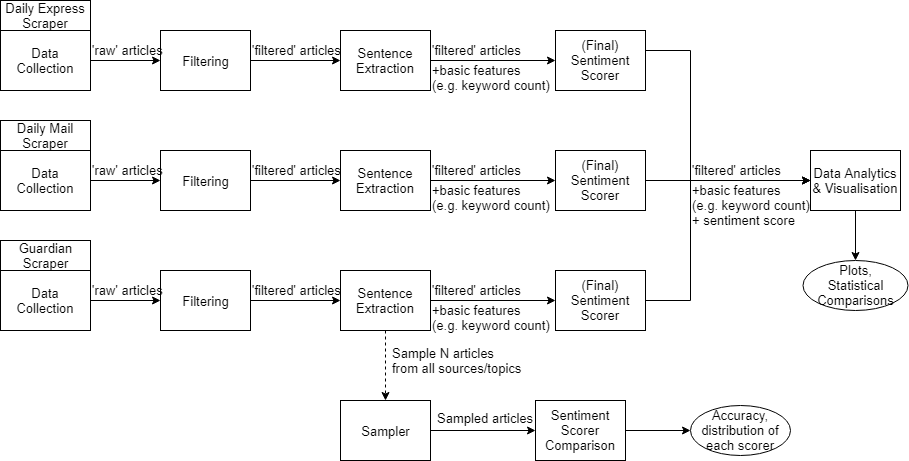
\includegraphics[width=\textwidth]{overall-design.png}

In this experiment, the pipeline is ran once for each source and topic, generating a dataset of all articles for the specified topic from the source with all extracted features, stored in a file.
The 'plot' component then loads these files and combines the dataset of all articles for every source within the same topic, and produces various plots to show trends within the topic, and statistical metrics for each possible subset within the topic.

% Input/output format (of JSON files) before/after each stage, how these files are stored (file structure and JSON structure)
Components pass datasets to each other by storing all information it extracts in a JSON format.
The output file of an earlier component is read as the input file for the next component, given the same source and topic.
The format of the output/input files is a collection of JSON objects, where each line consists of a single JSON object, and each JSON object represents a single article.
The JSON object contains a key-value pair for each extracted feature, and each component preserves the previous component's information (key-value pairs) while appending the object with additional key-value pairs for each feature it extracts.
This design ensures that in case computation is interrupted for any reason, the dataset generated by the previous component has already been saved to a file, and computation can restart from the interrupted component (without having to re-run previous components).

%% Include the database or storage representation. (Originally after component description)
\section{Dataset Description} \label{Dataset Description}  % What data have I got

\subsection{Sources} \label{sources}

% sources (Guardian, DM, DE), why
The Internet is an increasingly common medium for news publishers to publish news articles and for consumers to read these articles.
As of 2017, 64\% of British individuals read and/or download online news, newspapers or magazines, a sharp increase from 20\% in 2007 \cite{statista2018share}. 

The Daily Mail (\url{dailymail.co.uk}) and the Guardian (\url{theguardian.com}) are the two most visited news publisher's web sites as of 2016, with a monthly viewership of 11.85 and 10.05 million respectively \cite{statista2018newspaper}, and are the main subjects of this experiment.
Additonally, The Daily Express (\url{express.co.uk}), a slightly smaller newspaper with a monthly viewership of 2.67 million in 2016 \cite{statista2018newspaper}, is also added as a news source in this experiment, to control for source size and explore how the experiment performs with smaller sample sizes.
Furthermore, the Guardian provides an API \cite{guardian} and the Daily Mail and Daily Express provide advanced search tools \cite{daily-mail, daily-express} to query news articles from their websites, which prove useful in their respective data collection component's implementation, although the pipeline would work with any online news source that provides an internal search tool.
Thus, these three news publisher sources (Daily Mail, Guardian, Daily Express) were selected the main subjects of this experiment.

\subsection{Topics, keywords, key phrases, and query terms} \label{topics}

% List topics, keywords/phrases, query terms here
The final list of topics relevant to disabilities and people with disabilities, and the keywords, key phrases, and query terms deemed relevant to each topic, are: 

\begin{longtabu} to \textwidth { | X[l] | X[l] | X[l] | } 
	\hline
	Topic & Keywords and Key Phrases & Query Terms \\ 
	\hline
	'disabled' & 'disabled', 'disability', 'handicapped', 'cripple', 'invalid', 'accessible', 'ablism', 'ableism', 'differently abled' & 'disabled', 'disability', 'ablism', 'ableism', 'differently abled' \\ 
	\hline
	'autism' & 'autism', 'autistic', 'asperger\textbackslash's', 'ASD' & 'autism', 'autistic', 'asperger\textbackslash's', 'ASD' \\ 
	\hline
	'blind' & 'blind', 'blindness', 'blindism', 'visual impairment', 'partially sighted', 'vision loss' & 'blind', 'blindness', 'visual impairment', 'partially sighted', 'visually impaired' \\ 
	\hline
	'cerebral palsy' & 'cerebral palsy', 'spastic' & 'cerebral palsy', 'spastic' \\ 
	\hline
	'deaf' & 'deaf', 'deafness', 'hearing impaired', 'hard of hearing', 'hearing loss' & 'deaf', 'deafness', 'hearing impairment', 'hard of hearing', 'hearing impaired' \\ 
	\hline
	'developmental delay' & 'developmental delay', 'developmental disability', 'developmental disorder', 'learning disability', 'slow learner', 'retardation', 'intellectual disability' & 'developmental delay', 'developmental disability', 'developmental disorder', 'learning disability' \\ 
	\hline
	'dyslexia' & 'dyslexia', 'dyslexic' & 'dyslexia', 'dyslexic' \\ 
	\hline
	'epilepsy' & ''epilepsy', 'epileptic', 'seizure' & 'epilepsy', 'epileptic' \\ 
	\hline
	'mental illness' & 'mental illness', 'mental health', 'mental disability', 'mental disorder', 'mental issue', 'brain injured', 'brain injury', 'brain damaged', 'psychological', 'psychiatric', 'emotional disorder', 'behavioural disorder', 'retardation', 'intellectual disability', 'mentally ill', 'mentally disabled', 'mentally handicapped' & 'mental illness', 'mental health', 'mental disorder', 'mental disability', 'mentally ill', 'mentally disabled', 'mentally handicapped' \\ 
	\hline
	'mute' & 'mute', 'muteness', 'mutism', 'cannot speak', 'difficulty speaking', 'synthetic speech', 'non-vocal', 'non-verbal' & 'mute', 'muteness', 'mutism', 'non-verbal' \\ 
	\hline
	'paralysis' & 'paraplegic', 'quadriplegic', 'spinal cord', 'paraplegia', 'quadriplegia', 'paralysed', 'paralyzed', 'paralysis', 'crippled', 'leg braces', 'wheelchair' & 'paraplegic', 'quadriplegic', 'paraplegia', 'quadriplegia', 'paralysis' \\ 
	\hline
	'speech impairment' & 'speech impairment', 'stutter', 'speech disability', 'speech disorder', 'communication disability', 'difficulty speaking', 'language impairment', 'language disorder', 'language disability', 'speech impediment', 'stammer' & 'speech impairment', 'stutter', 'speech disorder', 'speech impediment' \\ 
	\hline
\end{longtabu}

% topics: collection of keywords & query terms (keywords minus potentially off topic terms / combinations)
This list of key terms was roughly based on guidelines from the Californian \cite{ca-guideline} and UK \cite{uk-guideline} governments (ignoring whether the term is considered 'appropriate' or 'inappropriate', as terms labelled 'inappropriate' are often still commonly used in the news, and relevant to consider when deciding whether an article is on-topic), with a few additions based on other commonly-used terms found on sampled articles from Daily Express, Daily Mail, and Guardian.
The list of query terms were based on the list of key words, with words/phrases that could have other meanings (or combinations of multiple common words) removed (unless the word/phrase is very commonly used to refer to the disability, such as 'blind' and 'mute').

\subsection{Dataset Size} \label{dataset-size}

% Tables for how many articles do I have, for each source, topic, and source+topic, before and after filtering
The dataset is comprised of all articles found online given the query terms defined in section \ref{topics}, published between 2000 to (approximately) late-March/early-April 2018.
The size of the initial collected dataset (i.e. all articles collected by the Data Collection component, prior to any further processing) in number of articles, for each source and topic, were:

\begin{center}
	\begin{tabu} to 1.0\textwidth { | X[c] | X[c] | X[c] | X[c] | X[c] | }
		\hline
		Topic & Daily Express & Daily Mail & Guardian & Total \\
		\hline
		Disabled & 16,818 & 24,768 & 30,598 & 72,184  \\
		\hline
		Autism & 988 & 6,035 & 5,780 & 12,803  \\
		\hline
		Blind & 9,467 & 23,616 & 32,307 & 65,390  \\
		\hline
		Cerebral Palsy & 509 & 1,995 & 1,569 & 4,073  \\
		\hline
		Deaf & 6,795 & 20,686 & 8,163 & 35,644  \\
		\hline
		Developmental Delay & 965 & 3,529 & 1,517 & 6,011  \\
		\hline
		Dyslexia & 283 & 938 & 1,980 & 3,201  \\
		\hline
		Epilepsy & 700 & 2,924 & 2,368 & 5,992  \\
		\hline
		Mental Illness & 8,102 & 38,273 & 29,831 & 76,206  \\
		\hline
		Mute & 1,541 & 2,312 & 4,764 & 8,617  \\
		\hline
		Paralysis & 711 & 4,346 & 3,879 & 8,936  \\
		\hline
		Speech Impairment & 1,777 & 2,994 & 1,357 & 6,128  \\
		\hline
		Total & 48,656 & 132,416 & 124,113 & 305,185  \\
		\hline
	\end{tabu}
\end{center}

After filtering, the size of the dataset that was plotted, in number of articles for each source and topic,  were:

% todo double check calculations
\begin{center}
	\begin{tabu} to 1.0\textwidth { | X[c] | X[c] | X[c] | X[c] | X[c] | }
		\hline
		Topic & Daily Express & Daily Mail & Guardian & Total \\
		\hline
		Disabled & 1,852 & 6,035 & 8,524 & 16,411  \\
		\hline
		Autism & 128 & 1,755 & 1,278 & 3,161  \\
		\hline
		Blind & 775 & 3,008 & 3,894 & 7,677  \\
		\hline
		Cerebral Palsy & 25 & 253 & 75 & 353  \\
		\hline
		Deaf & 114 & 747 & 901 & 1,762  \\
		\hline
		Developmental Delay & 5 & 130 & 447 & 582  \\
		\hline
		Dyslexia & 19 & 110 & 281 & 410  \\
		\hline
		Epilepsy & 58 & 740 & 374 & 1,172  \\
		\hline
		Mental Illness & 398 & 6,794 & 8,137 & 15,329  \\
		\hline
		Mute & 24 & 147 & 285 & 456  \\
		\hline
		Paralysis & 53 & 1,003 & 405 & 1,461  \\
		\hline
		Speech Impairment & 57 & 73 & 85 & 215  \\
		\hline
		Total & 3,508 & 20,813 & 24,646 & 48,967  \\ 
		\hline
	\end{tabu}
\end{center}

For the results evaluation, the focus will be on the 'disabled' topic, as it has the highest amount of news articles within its subset, and is the most generalisable topic on disabilities (as it refers to the general theme of disabilities and people with disabilities, rather than a specific topic).

\subsection{Limitations} \label{limitations}

% Limitations (e.g. DE has less articles than DM or Guardian, some topics have way less articles), implications for statistical analysis, plotting (e.g. moving averages), etc
As shown in section \ref{dataset-size}, the Daily Express has significantly less articles for any given topic than the Daily Mail or the Guardian, sometimes much less so.
Some topics, such as cerebral palsy, developmental delay, dyslexia, mute, and speech impairment, are also severely lacking in sample size of articles (post-filter).
In particular, cases where there are less than \textapprox200 articles for a source within a topic were problematic to plot or form statistically-significant conclusions regarding trends (e.g. to compare with other sources), as the distribution of the data is too varied. % todo redefine threshold based on Mann-Whitney U test results in chapter 5
In section \ref{Sentiment score: statistical comparison of different sources}, we show that it was difficult to obtain statistically significant conclusions when comparing to subsets with less than \textapprox200 articles.
This means that it is difficult to analyse or compare the Daily Express's subset for topics other than general 'disabled', 'blind', and 'mental illness', due to its relative lack of sample size.

% Also year-on-year limitations (DM only retains articles from ___, DE only retains articles from ___, Guardian only retains articles from ___), and implications (non equal proportion of articles for each year), what it means for analyses 
Another limitation with this experiment is the (limited) length of time each news source (Daily Express, Daily Mail, and Guardian) retain articles for in their online archive.
Our dataset indicates that by March/April 2018 (when this experiment took place), the Daily Express only retains articles from after \textapprox2007, the Daily Mail only retains articles from after \textapprox2010, and the Guardian only retains articles from after \textapprox2000. 
This raises an issue when analysing year-on-year trends, as the proportion of articles' sources within a topic are different in each year, and year-on-year differences may be better explained due to this difference in proportion, rather than an actual trend (see also: section \ref{Sentiment score: plots and trends}).
For this reason, we consider trends over time to be significant only when the trend is consistently repeated for each source's subset (instead of the full dataset for that topic), for all sources with statistically-significant sample size in that topic. 

\section{Components} \label{Components}
%% Give a description of the design of each of the components that make up the architecture.

\subsection{Data Collection}

% scraper for each source - what needs to be scraper from each article; article scraper AND search engine scraper

% crawler: use search engine scraper to get list of article URLs, use article scraper on each URL, store to JSON file line-by-line AND ensure ability to 'save and resume' and not repeat process for articles that already exist in the dataset (by loading a set of URLs that already exist in the dataset beforehand and not calling the scraper for them)

% mention how the requirement to resume on crash/interrupt led to saving a JSON object on each line (to represent each article) in the output so that articles are saved right after they are collected, not after all articles are collected - however, as a result, it violates the JSON standard (only one top-level object per file) - inconsequential but a drawback? regardless

\subsection{Dataset Filtering}

% What I did

% Evaluation of results - how I measured filter effectiveness & determine threshold rank

% Alternatives I considered

\subsection{Rule-based Sentence Matching}

% What I did

% Alternatives I considered

\subsection{Sentiment Scoring}

% short paragraph saying 'used open-source libraries' and 'several options were considered and their accuracy analysed on a random sample of sentences, before the two best-performing options were selected to be used for the full dataset, after being optimised for run-time (as running all options on the full dataset will take ~1 minute per article * 51,177 articles = ...)'

\subsubsection{Comparison of open-source implementations}

% a 'slow' scorer that takes the first N articles only and scores them with ALL scorers from a list of open-source sentiment scorers, for the purpose of evaluating the performance (accuracy) of these scorers

% Evaluation of results - how I measured model effectiveness (for each model)

% Graphs, Tables, analyses etc. expect like 2 pages

\subsubsection{Final implementation}

% After analysis, decided on running only two 'final' sentiment scorers for the whole dataset, using a separate function that computes only one sentiment score, optimised for performance (speed / runtime)

\subsection{Statistical Analysis and Visualisation}

% One sub-sub-section for each plot / analysis tool / metric being used (show data for 'disabled' and a few other examples from other keywords)

%% Provide implementation details as necessary.

%% As with other chapters, the structure and contents of this chapter will depend on the nature of your project, so the list above is only a suggestion, not a fixed requirement.

%% Find an ordering and form of words so that the design is clear, focusing on the interesting design decisions. For example, what were the alternatives, why select one particular solution? You have a limited number of pages so be selective about details. Also remember that someone (your examiners!) has to read this so don’t overwhelm them with intricate descriptions of everything that only you can follow – but do make sure the key details of the solution are in place. Use appropriate terminology and demonstrate that you have a good understanding of the Computer Science principles involved.

%% You can use diagrams and screen shots to help explain the design but don’t overuse them. Diagrams and screen shots should add information, not duplicate what is written in the text, and definitely avoid page after page of diagrams as this will disrupt the flow of your text. Where relevant, UML diagrams can certainly be used but, again, don’t flood the chapter with diagrams. Additional diagrams can always be included in an appendix section. It is not the case that a full set of UML diagrams must be provided for a software development project, and they shouldn’t be added in the belief that there must be UML diagrams to do a good project. Think about what you need to communicate and use UML diagrams if and when they fit the need.

%% It may be useful to include sections of code to highlight how a particular algorithm is implemented or how an interesting programming problem was solved. However, avoid lengthy sections of code, as this can also disrupt the flow of the text. Also make sure that your code fragments are readable, easy to follow and properly laid out. It may be better to use pseudo-code rather than actual code, especially when describing an algorithm. If you need to make use of longer sections of code, you can put the code in the appendix and reference it from the text.

%% An alternative way to organise the content of both this chapter and the preceding one, suitable for some projects, is to have a sequence of chapters or sections for each major iteration of the project. This allows the progression of the project to be shown, with each iteration building on the last, and the opportunity for interesting discussion about the decisions that needed to be made.

%% This is a core chapter in your report and will usually be quite substantial, 10 pages or more.


\chapter{Results Evaluation} \label{Results Evaluation}  % 2-4 pages (can be more if needed, probably more with graphs and tables)

\section{Focused topic} \label{Focused topic}
% This chapter will focus on the 'disabled' topic ... 
% Before going into sections, mention that although I have researched 12 topics relating to specific disabilities, this topic is chosen as an example for the resuls evaluation chapter as it is the most generic.
Although the pipeline was run on a list of twelve disability-related topics (as defined in section \ref{topics}), this results evaluation will mainly focus on the 'disabled' topic.
The 'disabled' topic was chosen as it has the highest amount of news articles within its subset, and it is the most generalisable topic (as it refers to the general theme of disabilities and people with disabilities, rather than a specific topic) (see also: section \ref{dataset-size}).
This focus on one topic for the whole of Chapter \ref{Results Evaluation} helps keep the numbers and results being discussed consistent throughout Chapter \ref{Results Evaluation}.
Furthermore, the full result plots for all topics will be available in the Appendix.

However, at several points in this chapter, results from other topics will also be discussed where it would add to the discussion.
Information from other topics will be explicitly mentioned (e.g. 'for the ... topic') such that the reader understands where the data does not refer to the 'disabled' topic.

% Explain the 'disabled' dataset first: provide a table with no. of articles for each source in each year.
Year-on-year trends are also a consistent theme throughout parts of this chapter.
Within the 'disabled' topic, the (post-filtering) sample size that was obtained for each year between 2000 and 2018 is as follows:

\begin{longtabu} to 1.0\textwidth { | X[c] | X[c] | X[c] | X[c] | X[c] | }
	\hline
	Year & Daily Express & Daily Mail & Guardian & Total \\
	\hline
	2000 & 0 & 0 & 504* & 504  \\
	\hline
	2001 & 0 & 0 & 294 & 294  \\
	\hline
	2002 & 0 & 0 & 334 & 334  \\
	\hline
	2003 & 0 & 2 & 330 & 332  \\
	\hline
	2004 & 0 & 2 & 387 & 389  \\
	\hline
	2005 & 0 & 0 & 381 & 381  \\
	\hline
	2006 & 0 & 0 & 338 & 338  \\
	\hline
	2007 & 51 & 0 & 424 & 475  \\
	\hline
	2008 & 86 & 0 & 424 & 510  \\
	\hline
	2009 & 175 & 0 & 352 & 527  \\
	\hline
	2010 & 157 & 173 & 365 & 695  \\
	\hline
	2011 & 166 & 370 & 607 & 1,143  \\
	\hline
	2012 & 238 & 516 & 822 & 1,576  \\
	\hline
	2013 & 133 & 473 & 638 & 1,244  \\
	\hline
	2014 & 140 & 846 & 544 & 1,530  \\
	\hline
	2015 & 177 & 1,095 & 526 & 1,798  \\
	\hline
	2016 & 260 & 1,128 & 640 & 2,028  \\
	\hline
	2017 & 220 & 1,094 & 506 & 1,820  \\
	\hline
	2018** & 49 & 336 & 108 & 493  \\
	\hline
	Total & 1,852 & 6,035 & 8,524 & 16,411  \\ 
	\hline
\end{longtabu}
*'2000' also includes a small amount of articles published before the year 2000.

**2018 is incomplete and would only include articles up to (approximately) late-March/early-April.

\section{Comparison of sentiment scorers} \label{Comparison of sentiment scorers}
% Short re-explanation of how these were compared, by taking a sample of 180? sentences, and manually labelling them, then plotting the sentiment-score distributions of 'positive' and 'negative' sentences for each scorer (summary of 4.3.4.1)

% results for how open-source sentiment scorers compare, plots, confusion matrices, accuracy, etc.

% discuss about how VADER, although much simpler than other models, is more generalisable than stat-ML/NN models trained on different domains

\section{Sentiment score: plots and trends} \label{Sentiment score: plots and trends}
% graphs, tables (mean std dev) relating to sentiment

\section{Sentiment score: statistical comparison of different sources} \label{Sentiment score: statistical comparison of different sources}
% Mann-Whitney U analysis (re-define it again, what it means for statistical significance etc)

% Table of Mann-Whitney U scores for each topic and source comparisons, overlap with n_articles for each source

% 

\section{Key terms: plots and trends} \label{Key terms: plots and trends}
% key terms analysis: most of them stay constant over the period (probably because 18 years data is quite short for cultural shifts), but mention the few where visible trends can be seen + show graphs. Also small sample sizes.
% also mention source-by-source variations

%% Describe your testing strategy (unit, functional, acceptance testing; and how they are carried out). How were test cases selected?
% Not Applicable

%% Examples of specific tests and how they were carried out (e.g., using mock objects to break dependencies). Focus on the interesting cases.
% Not Applicable

%% A summary of the test results and what coverage was achieved. Detailed test reports should appear in the appendix, if they add useful information or you want to demonstrate the kinds of tests and coverage achieved.
% Not Applicable

%% If your project requires substantial evaluation of data and results, evaluation of algorithms, or other forms of testing that are not code-based, then adapt this chapter to suit.
%% This chapter will typically be 2-4 pages in length but could be more depending on the depth of testing done. If you need to do a detailed evaluation for a more mathematical or theory-based project, then this chapter could well be more substantial.


\chapter{Conclusions} \label{Conclusions}  % 2-4 pages
%% Wrap-up and final thoughts on your project. 
%% This chapter is typically 2-4 pages long but could be longer if the project work requires more extensive evaluation.

\section{Achievements} \label{Achievements}
%% Summarise the achievements to confirm the project goals have been met.
%% A summary of what the project has achieved. Make sure that you address each goal set out in the Introduction chapter, to show that you have achieved what you claimed you would. Don’t leave any loose ends

\section{Evaluation} \label{Evaluation}
%% Evaluation of the work (this may be in a separate chapter if there is substantial evaluation).
%% A critical evaluation of the results of the project (e.g., how well were the goals met, is the application fit for purpose, has good design and implementation practice been followed, was the right implementation technology chosen and so on).

% Fit for purpose, but can still be improved (e.g. sentiment model would be much better using a more complex model trained on a similar domain, also code readability can be improved to make it a public library/API that everyone can understand, use, adapt - currently not very clear and sometimes reliant on commenting code out/in or changing values

% Choice of technologies (what's good e.g. Python, range of libraries, plotting, etc.; what can be improved i.e. try other methods e.g. topic models for filtering, inconsistency of models used e.g. stemming with NLTK for filtering vs lemmatising with SpaCy for rule-based sentence matching)

% Implications of NLP for future media studies, call for similar analyses to be conducted in other domains (mention additional information that can be discovered by using computational NLP and processing a much larger sample of text) 

\section{Future Work} \label{Future Work}
%% How the project might be continued, but don't give the impression you ran out of time!
%% Future work. How could the project be developed if you had another 6 months. Take care to differentiate between what you have done to satisfy your stated project goals, and work that could be done to meet extended goals.

% Purpose built sentiment model trained to a a labelled sample: in this analysis vader performed best although it's a very simple model as other, more complex pre-trained models were trained on other domains and is less generalisable. However, OpenAI's model came very close despite this, and a similar approach using deep learning or statistical ML models, trained on a labelled sample of positive/negative/neutral sentences in this domain, would have much improved sentiment score reliability (and thus quality of analyses)

% Expand sources - Develop API where others can use and adapt the code, change topics / keywords / key phrases / query terms, add/change sources by developing their own scrapers (with an interface for the scraper), document code and improve code readability and output file structure, output sample on-topic/off-topic articles to help them set rank threshold, maybe even an API to provide their own sentiment model(s) as parameter given an interface


\appendix

\printbibliography[heading=bibintoc]

\chapter{Other appendices, e.g., code listing}  % appendix A
\emph{Put your appendix sections here}

% \chapter{Test Appendix B}

\end{document}